%%%%%%%%%%%%%%%%%%%%%%%%%%%%%%%%%%%%%%%%%%%%%%%%%%%%%%%%%%%%%%%%%%%%%%%%%%%%%%%%
% Thesis / Project Report
% LaTeX Template
% Version 2.0 (08/04/16)
%
% Author:
% Siddhant Shrivastava
% https://github.com/sidcode/bits-pilani-thesis-template-latex
%
% This template is heavily based on the work of Darshit Shah, Steven Gunn and Sunil Patel
% Darshit Shah
% https://github.com/darnir/BPHC-LaTeX-Report-Class
% Steven Gunn
% http://users.ecs.soton.ac.uk/srg/softwaretools/document/templates/
% and
% Sunil Patel
% http://www.sunilpatel.co.uk/thesis-template/
%
% License:
% CC BY-NC-SA 4.0 (http://creativecommons.org/licenses/by-nc-sa/4.0/)
%
% Note:
% Make sure to edit document variables in the Thesis.cls file
%
%%%%%%%%%%%%%%%%%%%%%%%%%%%%%%%%%%%%%%%%%%%%%%%%%%%%%%%%%%%%%%%%%%%%%%%%%%%%%%%%

%-------------------------------------------------------------------------------
%	PACKAGES AND OTHER DOCUMENT CONFIGURATIONS
%-------------------------------------------------------------------------------

\documentclass[11pt, a4paper, oneside]{Thesis} % Paper size, default font size
                                               % and one-sided paper

\graphicspath{{Pictures/}} % Specifies the directory where pictures are stored

\title{\ttitle} % Defines the thesis title - don't touch this

\begin{document}

\frontmatter % Use roman numbering style (i, ii...) for the pre-content pages

\setstretch{1.5} % Line spacing required for the submitted report

% Define page headers using FancyHdr package and set up for one-sided printing
\fancyhead{} % Clears all page headers and footers
\rhead{\thepage} % Sets the right side header to show the page number
\lhead{} % Clears the left side page header

\pagestyle{fancy} % Finally, use the "fancy" page style to implement the
                  %FancyHdr headers

% Input all the variables used in the document. Please fill out the
% variables.tex file with all your details.
%-------------------------------------------------------------------------------
%	DOCUMENT VARIABLES
%
%	Fill in the lines below to set the various variables for the document
%-------------------------------------------------------------------------------

%-------------------------------------------------------------------------------
% Your thesis title - this is used in the title and abstract
% Command: \ttitle
\thesistitle{IronClaw: Dynamic Tool Synthesis and Secure MicroVM Isolation for Autonomous Agents}
%-------------------------------------------------------------------------------
% The document type: Thesis / report, etc.
% Command: \doctype
\documenttype{Undergraduate Thesis}
%-------------------------------------------------------------------------------
% Your supervisor's name - this is used in the title page
% Command: \supname
\supervisor{Dr. Vijaykumar B.}
%-------------------------------------------------------------------------------
% The supervisor's position - Used on Certificate
% Command: \suppos
\supervisorposition{Faculty}
%-------------------------------------------------------------------------------
% Supervisor's institute
% Command: \supinst
\supervisorinstitute{BITS Pilani}
%-------------------------------------------------------------------------------
% Your Co-Supervisor's name
% Command: \cosupname
\cosupervisor{}
%-------------------------------------------------------------------------------
% Co-Supervisor's Position - Used on Certificate
% Command: \cosuppos
\cosupervisorposition{}
%-------------------------------------------------------------------------------
% Co-Supervisor's Institute
% Command: \cosupinst
\cosupervisorinstitute{}
%-------------------------------------------------------------------------------
% Your Examiner's name. Not currently used anywhere.
% Command: \examname
\examiner{}
%-------------------------------------------------------------------------------
% Name of your degree
% Command: \degreename
\degree{Bachelor of Engineering (Hons.)}
%-------------------------------------------------------------------------------
% The BITS Course Code for which this report is written
% COmmand: \ccode
\coursecode{BITS F423T}
%-------------------------------------------------------------------------------
% The name of the Course
% Command: \cname
\coursename{Thesis}
%-------------------------------------------------------------------------------
% Your name. Extend manually in case of multiple authors
% Command: \authornames
\authors{Suryavir Kapur}
%-------------------------------------------------------------------------------
% Your ID Number - used on the Title page and abstract
% Command: \idnum
\IDNumber{2022A7TS0293U}
%-------------------------------------------------------------------------------
% Your address
% Command: \addressnames
\addresses{}
%-------------------------------------------------------------------------------
% Your subject area
% Command: \subjectname
\subject{Autonomous agents, microVM isolation, dynamic tool synthesis}
%-------------------------------------------------------------------------------
% Keywords for this report.
% Command: \keywordnames
\keywords{IronClaw, autonomous agents, large language models, dynamic tool synthesis, Firecracker, microVMs, sandboxing, vsock}
%-------------------------------------------------------------------------------
% University details
% Command: \univname
\university{\texorpdfstring{\href{http://www.bits-pilani.ac.in/}
                {Birla Institute of Technology and Science Pilani}}
                {Birla Institute of Technology and Science Pilani}}
%-------------------------------------------------------------------------------
% University details, in Capitals
% Command: \UNIVNAME
\UNIVERSITY{\texorpdfstring{\href{http://www.bits-pilani.ac.in/}
                {BIRLA INSTITUTE OF TECHNOLOGY AND SCIENCE PILANI}}
                {BIRLA INSTITUTE OF TECHNOLOGY AND SCIENCE PILANI}}
%-------------------------------------------------------------------------------
% Department Details
% Command: \deptname
\department{\texorpdfstring{\href{http://www.bits-pilani.ac.in/pilani/computerscience/ComputerScience} % Your department's URL
                {Computer Science \& Information Systems}} % Your department's name
                {Computer Science}}
%-------------------------------------------------------------------------------
% Department details, in Capitals
% Command: \DEPTNAME
\DEPARTMENT{\texorpdfstring{\href{http://www.bits-pilani.ac.in/pilani/computerscience/ComputerScience} % Your department's URL
                {COMPUTER SCIENCE \& INFORMATION SYSTEMS}} % Your department's name in capitals
                {COMPUTER SCIENCE \& INFORMATION SYSTEMS}}
%-------------------------------------------------------------------------------
% Research Group Details
% Command: \groupname
\group{Autonomous Systems and Security}
%-------------------------------------------------------------------------------
% Research Group Details, in Capitals
% Command: \GROUPNAME
\GROUP{AUTONOMOUS SYSTEMS AND SECURITY}
%-------------------------------------------------------------------------------
% Faculty details
% Command: \facname
\faculty{Computer Science}
%-------------------------------------------------------------------------------
% Faculty details, in Capitals
% Command: \FACNAME
\FACULTY{COMPUTER SCIENCE}
%-------------------------------------------------------------------------------

%-------------------------------------------------------------------------------
%   NON-CONTENT PAGES
%-------------------------------------------------------------------------------
\maketitle
\Declaration
\Certificate
\Quotation{Security is a process, not a product.}{Bruce Schneier}

\begin{abstract}
As Large Language Models (LLMs) continue to grow as agents capable of performing ever increasing numbers of increasingly complex, multi-step workflows, these models typically have access to relatively small sets of static, pre-defined, or "fixed" toolsets. If we allow LLM agents to create, and subsequently run, task-specific tools at runtime, this will significantly enhance their ability to perform long-horizon software development and data processing work; however, executing synthesized code in ordinary, process level sandboxes creates significant potential security risk. This dissertation will introduce and describe IronClaw -- an autonomous agent platform that provides both dynamically created tools and strictly isolated Firecracker micro-VMs. In other words, IronClaw separates the host daemon, responsible for managing agent policy, context and lifecycle management from a guest runtime where the agent generates untrusted code to be executed behind a hardware-based virtualization barrier.

The evaluation methodology described herein is based on assessing whether the generation of tools dynamically relative to the use of fixed toolsets enhances the effectiveness of autonomous agent utility. Additionally, the trade-off's associated with using micro-VM isolation versus running agent generated tools in a process sandbox environment are evaluated in terms of security and performance. A complex set of software engineering and data transformation tasks are used to evaluate the effectiveness of each mode. Red teaming style prompts designed to cause host escape and/or resource exploitation are also used to assess the relative strengths/weaknesses of the two environments. Latency, CPU usage, and memory utilization overhead measurements are taken across the three execution modes to provide additional insight into differences between them. Ultimately, the goal of this research is to produce a repeatable evaluation of whether dynamic tool synthesis for secure operation can be made practically viable for autonomous agents while maintaining effective containment of the host system.
\end{abstract}

\begin{acknowledgements}
This thesis would not have been possible without the patient guidance of my supervisor, Dr. Vijaykumar B., whose thoughtful suggestions and steady encouragement carried me through every stage of this work, and without the stimulating academic environment provided by the Department of Computer Science and Information Systems at BITS Pilani, where the ideas behind IronClaw were explored, refined, and brought to life. Equally, I am grateful to my family and friends, who gave so freely of their time in testing the system, shaping its documentation, and supporting its development, and whose quiet belief in this work sustained me throughout.
\end{acknowledgements}

%-------------------------------------------------------------------------------
%	LIST OF CONTENTS/FIGURES/TABLES PAGES
%-------------------------------------------------------------------------------

% The page style headers have been "empty" all this time, now use the "fancy"
% headers as defined before to bring them back
\pagestyle{fancy}

\lhead{\emph{Contents}} % Set the left side page header to "Contents"
\tableofcontents % Write out the Table of Contents

% Set the left side page header to "List of Figures"
\lhead{\emph{List of Figures}}
\listoffigures % Write out the List of Figures

 % Set the left side page header to "List of Tables"
\lhead{\emph{List of Tables}}
\listoftables % Write out the List of Tables

%-------------------------------------------------------------------------------
%	ABBREVIATIONS
%-------------------------------------------------------------------------------

\clearpage % Start a new page

 % Set the line spacing to 1.5, this makes the following tables easier to read
\setstretch{1.5}

\lhead{\emph{Abbreviations}} % Set the left side page header to "Abbreviations"
\listofsymbols{ll} % Include a list of Abbreviations (a table of two columns)
{
\textbf{API} & \textbf{A}pplication \textbf{P}rogramming \textbf{I}nterface \\
\textbf{LLM} & \textbf{L}arge \textbf{L}anguage \textbf{M}odel \\
\textbf{VMM} & \textbf{V}irtual \textbf{M}achine \textbf{M}onitor \\
\textbf{VM} & \textbf{V}irtual \textbf{M}achine \\
\textbf{vsock} & \textbf{V}irtual socket transport \\
}

%-------------------------------------------------------------------------------
%	PHYSICAL CONSTANTS/OTHER DEFINITIONS
%-------------------------------------------------------------------------------

\clearpage % Start a new page

% Set the left side page header to "Physical Constants"
\lhead{\emph{Physical Constants}}

 % Include a list of Physical Constants (a four column table)
\listofconstants{lrcl}
{
Target microVM initialization latency & $t_{init}$ & $<$ & 500 ms \\
Maximum tool execution time & $t_{exec}$ & $=$ & policy-defined \\
Maximum tool output size & $s_{out}$ & $=$ & policy-defined \\
}

%-------------------------------------------------------------------------------
%	SYMBOLS
%-------------------------------------------------------------------------------

\clearpage % Start a new page

\lhead{\emph{Glossary}} % Set the left side page header to "Symbols"

\listofnomenclature % List the nomenclature. (We use the glossaries package)

%-------------------------------------------------------------------------------
%	DEDICATION
%-------------------------------------------------------------------------------

\setstretch{1.3} % Return the line spacing back to 1.3

\pagestyle{empty} % Page style needs to be empty for this page

% Dedication text
\Dedicatory{Dedicated to my family, mentors, and peers.}

\addtocontents{toc}{\vspace{2em}} % Add a gap in the Contents, for aesthetics

%-------------------------------------------------------------------------------
%	THESIS CONTENT - CHAPTERS
%-------------------------------------------------------------------------------

\mainmatter % Begin numeric (1,2,3...) page numbering

\pagestyle{fancy} % Return the page headers back to the "fancy" style

% Include the chapters of the thesis as separate files from the Chapters folder
% Uncomment the lines as you write the chapters

% Chapter 1

\chapter{Introduction}
\label{Chapter1}
\lhead{Chapter 1. \emph{Introduction}}

\section{Background}
Large Language Model-based autonomous agents are being widely applied in a variety of domains for long-range tasks including software support, data management, documentation processing and process automation. In many cases these agents use static registries of pre-defined tools provided to them from their developer. While this approach has advantages relative to auditing and permissioning; it severely limits the ability of the agent to perform tasks that require intermediate parsers, converters, benchmarks and integrations that were not provided prior to the beginning of the task.

The goal of dynamic tool synthesis is to provide agents the ability to dynamically create new capabilities by executing small programs, examining their results, and using those results as a capability for performing a particular type of task. However, the generation of new capabilities changes the underlying security model. It is possible for generated capabilities to include maliciously intended destructive operations, command injection prompts, resource consumption attacks, or deliberately designed host escapes. Therefore, simply sandboxing the process hosting the agent is often insufficient protection against maliciously generated code created during an open-ended conversation.

IronClaw addresses the challenge of integrating dynamic tool synthesis with Firecracker microVM isolation. The host process manages policy, LLM context, and microVM lifecycle decisions. Untrusted tool code runs in a guest runtime within a microVM. Data exchange occurs over a controlled transport boundary, allowing the system to return tool results without providing generated code with direct access to host resources.

\section{Use Cases}
IronClaw is designed for scenarios where autonomous agents need to solve tasks
that go beyond what a fixed registry of tools can handle while keeping host
systems secure. Here are some examples of tradeoffs that motivate the design.

\subsection{Ad Hoc Data Transformation}
Agents frequently encounter files or streams in formats for which no
pre-installed tool exists. For example, users might ask the agent to extract
metrics from custom log formats, convert between domain specific serialization
formats, or aggregate columns from several inconsistent CSV files. IronClaw can
synthesize small parsers or transformers and run them inside micro VMs.
Boundaries of this VM ensure that malformed or malicious transformations cannot
read host filesystem or leak data.

\subsection{Sandboxed Analysis of Untrusted Artifacts}
Security and incident response workflows often require analyzing files that
themselves might be hostile such as suspicious scripts, downloaded executables
or email attachments Rather than exposing hosts to artifacts, agents can
generate analysis tools and send approved explicit inputs to guests and observe
bounded outputs. If generated code tries to breach containment, it stays
confined to disposable guest environment.

\subsection{Dynamic Integration of APIs and Services}
An agent may encounter an external API for which no purpose-built capability is
available. It can then generate a minimal HTTP client or SDK wrapper on demand.
IronClaw runs generated clients in the guest with network policies enforced by
the host and thus integrates without giving tools persistent network privileges
on the host.

\subsection{Iterative Code Generation and Testing}
Often software engineering tasks require writing, running and refining small
programs. IronClaw lets agents generate candidate code and execute unit tests or
benchmarks in the guest and observe failures and then iterate. Each execution
runs in an isolated guest so buggy code or hostile code cannot corrupt workspace
on the host or persist between iterations.

\section{Problem Statement}
This dissertation asks whether autonomous agents gain measurable utility by
synthesizing and reusing their own tools while maintaining strong separation
from the host. When no purpose-built capability is available, repeatedly
authoring task logic inline may consume additional model steps and tokens.
Dynamic synthesis may avoid that repeated effort, but generated code increases
the risk to the host. IronClaw makes this utility/security trade-off measurable
by comparing no synthesis with dynamic synthesis for utility, and ordinary
process execution with microVM execution for containment and systems cost.

\section{Objectives}
The objectives of this thesis are:
\begin{itemize}
    \item To design and implement a dynamic execution path for agent-generated
    tools in IronClaw.
    \item To isolate untrusted generated code using Firecracker microVMs and a
    strict host/guest boundary.
    \item To compare agents with dynamic tool synthesis against otherwise
    equivalent agents that must author task logic inline on every request.
    \item To evaluate containment against simulated malicious generated tools.
    \item To profile the latency and resource overhead introduced by microVM
    isolation.
\end{itemize}

\section{Research Questions}
This thesis is guided by the following research questions:
\begin{itemize}
    \item \textbf{RQ1: Utility.} On repeated, complex tasks for which no
    purpose-built tool is available, does dynamic tool synthesis reduce agent
    interaction steps and token consumption relative to authoring the required
    logic inline, without reducing answer correctness?
    \item \textbf{RQ2: Security and Systems.} What is the measurable security
    containment capability and performance overhead of Firecracker microVM
    isolation compared to traditional process-level sandboxing when executing
    agent-generated code?
\end{itemize}

\section{Hypotheses}
The thesis evaluates two hypotheses:
\begin{itemize}
    \item \textbf{H1: Utility.} On repeated tasks for which no purpose-built
    tool is available, policy-guided dynamic tool synthesis reduces model
    interaction steps and token consumption relative to generic capabilities
    alone, while preserving task correctness. The benefit increases with reuse.
    \item \textbf{H2: Security and Performance.} IronClaw's microVM architecture
    contains simulated host-breakout attempts from malicious synthesized tools,
    at the cost of measurable but acceptable initialization latency and memory
    overhead.
\end{itemize}

% Chapter 2

\chapter{Literature Review and Background}
\label{Chapter2}
\lhead{Chapter 2. \emph{Literature Review and Background}}

\section{LLM Agents and Tool Use}
LLM agents extend language models by allowing them to call external tools,
maintain task state, and decompose goals into multi-step plans. Tool use improves
reliability because the model can delegate exact computation, file operations,
search, or program execution to deterministic systems. ReAct-style prompting
demonstrated that interleaving reasoning traces with actions can improve
interactive task solving \cite{yao2023react}. Toolformer showed that language
models can learn to decide when external API calls are useful
\cite{schick2023toolformer}. Generative Agents demonstrated memory, reflection,
and planning loops for believable software agents \cite{park2023generative},
while Voyager showed how an LLM agent can accumulate executable skills in an
open-ended environment \cite{wang2023voyager}.

Although a lot of progress has been made toward developing the ability for deployed agents to create tools with some degree of flexibility, most still rely on static registries of tools created before they begin a particular task. This type of static registry makes auditing easier; however, since the agent cannot create new utilities while performing a task (i.e., during runtime), this can severely limit its capabilities. Dynamic Tool Synthesis (DTS) allows an agent to develop small programs for task-specific transformations, tests, or integrations at runtime using dynamic tool synthesis.

\section{Dynamic Tool Synthesis}
The primary reason DTS is useful when there are specific tasks where code creation is unpredictable in advance (e.g., converting files in unknown formats, aggregating results from benchmarks, validating various configuration options, creating domain-specific checks). The process begins with the agent writing code. Once the agent creates the code, the agent then runs the code in an isolated environment. Following execution of the code by the agent, the agent then reviews the output of the executed code and determines if it should revise or reuse the newly developed tool.

\section{Sandboxing and Isolation}
Traditional sandboxing techniques include language-level restrictions,
process-level privilege dropping, containers, seccomp filters, and namespaces.
These controls reduce the attack surface but still share the host kernel. A
kernel vulnerability or misconfiguration can turn a process-level boundary into a
host compromise. MicroVMs provide a stronger boundary by running guest workloads
inside hardware-assisted virtualization while retaining low startup overhead
compared with general-purpose virtual machines. This design follows the classic
virtual-machine monitor goal of providing equivalent execution, resource
control, and efficiency as formalized by Popek and Goldberg
\cite{popek1974formal}.

\section{Fundamentals of Sandboxing}
Sandboxes are systems where code is executed in an "environment" (a sandbox) with restrictions on what it can do. These restrictions include limiting file access, restricting network activity, constraining cpu & memory usage, restricting system calls, and limiting execution time.

Agent generated code should never be treated as a convenience item, but as a required security mechanism. The model could produce code that is syntactically correct but semantically dangerous. In addition, the model could take malicious instructions from outside the system. As such, the sandbox must consider all code produced by the model to be malicious regardless of whether the end-users' requests were benign.

\section{Processes, Containers, and Virtual Machines}
An operation that is completely separate to other operations (i.e. it cannot interact with them) will be provided by the operating systems "memory management" and "permission" models. This is a good thing as the process can run independently, however, in order to have some commonality (in terms of how the kernel executes), all processes share the same kernel on their host. Therefore if there is a bug within the host kernel, a mis-configuration of permissions, etc., then the host could potentially be compromised due to an attack upon the process.

Namespaces, cgroups, capabilities, and file-system layering provide an additional layer of abstraction around processes so that each container runs in isolation from one another. Containers are also very efficient and practical for providing packages around an applications workload. However, containers do not create a complete hardware boundry for the workload, since the workload continues to run using the host kernel. This would present issues with IronClaw since generated tools are not typical application code. Rather they are generated code that was created at runtime which would be un-trusted code.

A Virtual Machine (VM) creates a stronger boundry than a Container. Since VMs use virtualized hardware to run a Guest Operating System, the Guest OS operates under its own kernel. Also, the Guest has its own memory view, devices and process tree. It is not possible for the Host Kernel to run Guest OS commands. Rather, when the Guest OS wishes to perform privileged functions these are mediated through a Hypervisor or Virtual Machine Monitor. By separating the Host and Guest OSes this limits the Blast Radius of Un-Trusted Code. That is, a compromise of a Guests OS would not immediately result in a Host compromise. Xen is a canonical example of a virtual machine monitor designed to
run multiple commodity operating systems safely on shared hardware
\cite{barham2003xen}.

\section{How Virtual Machines Execute on the CPU}
The architecture of modern CPU’s includes hardware extensions that enable a hypervisor to execute guest code in an efficient manner (Intel VT-x and AMD-V). The Architecture Manuals for Intel detail the VMX root and non-root modes that are utilized to enter, run, exit, and resume virtual machines. A simple view of the CPU is that there are two main execution modes; a host-controlled mode for the hypervisor and a guest-mode for the virtual machine. Most ordinary instructions executed by the guest will be executed directly on the CPU. Thus, a virtual machine is not just an emulator, running every instruction.

When guest-code performs some type of sensitive operation that would alter privileged CPU state, access certain devices, etc., the CPU will perform a VM Exit. At this point, control will pass back to the hypervisor who can determine how to process the request. Once processed, the hypervisor can then resume the guest with a VM Entry. This exit-and-entry paradigm enables normal computations to run at near-native speeds, while still keeping all privileged actions under host-control. Research has shown that performance in virtualized environments can be greatly impacted by the number and duration of VM Exits, page table entries/updates, and I/O transactions \cite{adams2006comparison}.

Hardware-based support is also available to help enforce memory isolation between different guests and their respective hypervisors. Each guest operating system believes it is controlling its own set of physical memory locations. However, these guest-physical memory locations are actually mapped to host-physical memory pages via mechanisms such as Extended Page Tables (EPT) on Intel processors or Nested Page Tables (NPT) on AMD processors. These mappings prevent each guest from directly writing to or reading from any arbitrary portion of the hosts' physical memory.

\begin{figure}[htbp]
    \centering
    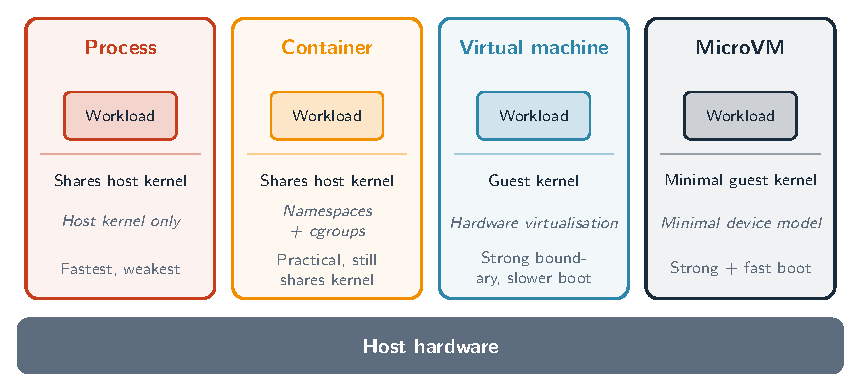
\includegraphics[width=0.95\linewidth]{Figures/fig_isolation_boundaries.pdf}
    \caption{Sandboxing isolation continuum, comparing process, container, virtual machine, and microVM boundaries.}
    \label{fig:isolation_boundaries}
\end{figure}

\fref{fig:isolation_boundaries} summarises the differences between the
sandboxing approaches discussed above.

\section{MicroVMs}
A microVM is a virtual machine designed with a deliberately small device model
and minimal management surface. It keeps the stronger hardware virtualization
boundary of a VM while reducing the startup time and attack surface associated
with traditional general-purpose virtual machines. What is done here is basically instead
of passing in all available PCIe devices, we only pass in the devices that are needed for
the workload, in our case only usually network and disk. This makes microVMs suitable
for short-lived, isolated workloads such as serverless functions and
agent-generated tools. Firecracker is a production example of this approach,
designed specifically for lightweight virtualization in serverless applications
\cite{agache2020firecracker}.

In IronClaw, a microVM can be created for a tool execution or task session, run
the generated code, return bounded output, and then be discarded. This ephemeral
model helps prevent persistence, cross-tool contamination, and accidental reuse
of compromised state.

\section{Firecracker MicroVMs}
The Firecracker project implements a lightweight Virtual Machine Monitor (VMM)
which supports secure multi-tenancy, as well as providing a minimalist device
model with fast start up capabilities. These features make it particularly
suited for short-lived isolated task. IronClaw uses Firecracker to execute
agent generated code within an ephemeral environment in order to isolate
the execution of the tools from the host daemon, which also enables the host
to delete or recreate the guest runtime at the end of every session.

\section{Evaluation Benchmarks}
As part of its evaluation process, IronClaw will use complex software engineering
benchmarks similar to SWE-bench \cite{swebench}, however instead of evaluating
whether agents can reason over actual repository sources and provide accurate
fixes, the benchmarks will be focused on those tasks that are most likely to
be assisted by tool generation. Examples include: parsing output, executing
checks against specific inputs, transforming data, and repeatedly verifying
results.

% Chapter 3

\chapter{System Architecture}
\label{Chapter3}
\lhead{Chapter 3. \emph{System Architecture}}

\section{Overview}
IronClaw is an autonomous-agent hosting platform that has a very strict host / guest split. The host process (daemons), ironclawd, is responsible for all of the "privileged" things in the system; these include loading the configuration file, enforcing policies, managing memory, interacting with large language models (LLM), and controlling the lifecycle of micro-VMs. The guest runtime, irowclaw, is executing within a Firecracker boundary and will execute untrusted tool requests coming from the host.

This design was intended to be asymmetric. The host is assumed to be trusted and stateful: it maintains the conversation state, holds onto long-term configurations, makes decisions about what tools are allowed, and retains connections to external model providers. Conversely, the guest is intentionally small and ephemeral: it accepts bounded executions on behalf of the host, run those executions against a set of policies, returns structured data back to the host and can be discarded once it's completed its task. This separation allows the complex logic for controlling agents to exist in a trusted location away from the potentially un-trusted execution environment while also prevents synthesized tools from being able to access resources held by the host workspace.

\begin{figure}[htbp]
    \centering
    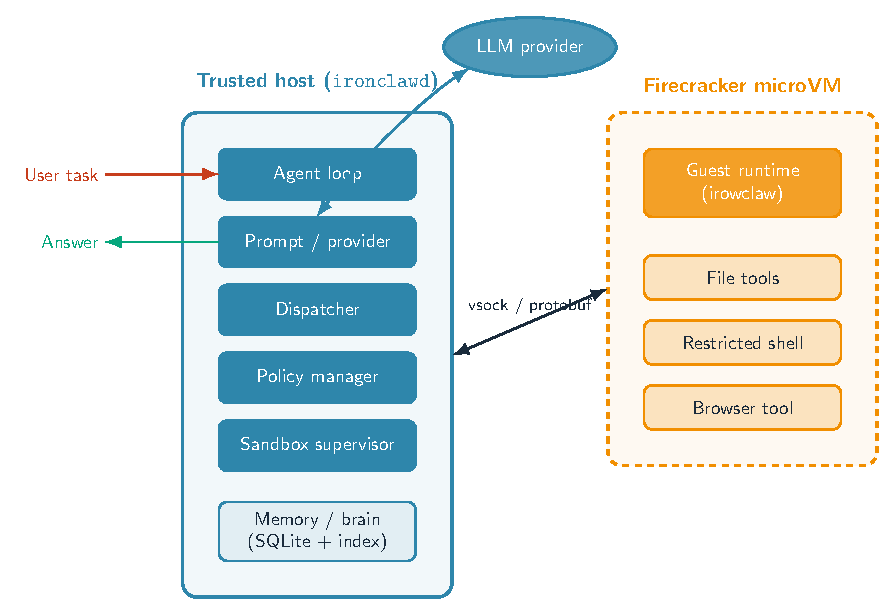
\includegraphics[width=0.95\linewidth]{Figures/fig_architecture.pdf}
    \caption{IronClaw host/guest architecture: the trusted host daemon manages the agent loop and sandbox lifecycle, while generated tools execute inside a Firecracker microVM guest runtime.}
    \label{fig:architecture}
\end{figure}

\fref{fig:architecture} shows the resulting host/guest split.

\section{Host Daemon}
In addition to starting and stopping Guest Runtimes, the Host Daemon also has control of what capabilities are enabled during a Session. The Host receives the User's Tasks, generates Model Prompts based on Task Context, Memory, Tool Results and Policy Reminders, Dispatches Tool Calls, and records Memory Usage.

Since Generated Tools are considered Un-trusted, the Host does not execute them. The Host Packages the Tool Specification and Code in order to have that executed by the Guest Runtime.

There are five Subsystems that work together Internally to allow the Host Daemon to Function. There is an Agent Loop that Maintains the Plan-Act-Observation Cycle, and determines if the Next Action is a Fixed Tool Call, a Generated Tool, or Final Answer. There is a Prompt/Provider Layer that Builds Model Prompts based on Task Context, Memory, Tool Results and Policy Reminders, and sends those Prompts to the Configured LLM Provider. There is a Dispatcher that Normalizes Model Actions into Typed Execution Requests, and Routes those Typed Execution Requests to either Local Fixed Tools, or the Guest Runtime. There is a Policy Manager that Determines Limits for Filesystem Access, Network Access, CPU Time, Memory, Output Size and Allowed Interpreters. Finally, there is a Sandbox Supervisor that Creates, Monitors/Times Out/Destroys Guest Runtimes.

Additionally, the Host Daemon performs Result Triage. A Response from a Guest Runtime is not simply Replaced Back into the Model Context. Rather it is Bounded, Decoded, Tagged with Status Metadata Summarized Where Necessary to prevent Destabilization of the Next Agent Turn due to Large Outputs or Malformed Responses.

\section{Guest Runtime}
The guest runtime is much smaller in size than the host. It accepts execution requests from the host, validates the request envelope (to ensure integrity), runs allowed commands or generates tool code based on the input provided in the request, captures standard output and error from the command or code that was run, and returns structured results back to the host.
This is done by placing a guest runtime inside an ephemeral Firecracker microVM so that file system changes, process state, memory effects are confined to the guest session only.

There are three main responsibilities of the guest runtime.

Firstly it verifies whether the request sent by the host matches expected protocol & required fields such as: request identifier, tool name, input payload, & execution limits are present.

Secondly it creates the execution environment for the guest runtime which includes creating/populating files necessary for the tool execution, selecting the interpreter or binary path used for execution, applying local process limitations.

Thirdly it catches the result of the execution of the tool as a structured response containing exit status, stdout, stderr, duration of execution & error classification.

A guest should not be responsible for holding secrets, long-term credentials or broader host mounts. All data needed for the execution of a tool will be explicitly sent by the host with each request. This makes reasoning about what the guest can see much simpler: if a payload tries to inspect the system it should only see the minimal guest file system & only the inputs specifically provided for that single run.

\section{Transport Boundary}
IronClaw uses a controlled host/guest communication path. The project includes
vsock transport components and smoke tests for Firecracker round trips. The
transport is responsible for carrying execution requests into the guest and
returning bounded outputs to the host. This boundary is a key part of the
security model because the host exposes only the protocol surface required for
tool execution.

The request envelope is designed to be explicit rather than shell-like. A
typical execution request contains:
\begin{itemize}
    \item a unique request identifier for correlating logs and responses;
    \item the declared tool name and tool type;
    \item code or command material to be executed;
    \item serialized input parameters and optional input files;
    \item policy fields such as timeout, memory limit, network mode, and output
    limit;
    \item an expected result format such as text, JSON, or file artifact.
\end{itemize}

The response mirrors the same structure. It includes the request identifier,
success or failure status, exit code, stdout, stderr, duration, and any produced
artifact metadata. This structure is important because it lets the host handle a
timeout, policy denial, runtime crash, or successful result differently instead
of treating every guest response as plain text.

\section{Dynamic Execution Engine}
The runtime dynamically runs tools that have been created by the agent running. Tool requests contain the name of the tool, what the user intends for the tool to do, the code (executable) to be run with in the isolated runtime, input parameters for the code, and any execution constraints on how the code should execute. The guest takes the code and either interprets or compiles it inside the isolated runtime, then executes it. Once executed, the guest sends the results back to the agent. If there is an error when executing a tool, the agent will receive the failure as structured error information; this allows the agent to potentially correct the creation of the tool, or use a fixed capability instead.

The dynamic execution loop proceeds in six stages:
\begin{enumerate}
    \item The agent identifies that no fixed tool is sufficient for the current
    subtask.
    \item The model proposes a small tool with a purpose, inputs, and code.
    \item The host validates the tool specification against policy and rejects
    unsafe requests before guest execution.
    \item The guest runs the tool in the microVM and captures bounded outputs.
    \item The host classifies the result as success, tool error, policy error,
    timeout, or infrastructure error.
    \item The agent observes the result and either continues the task, revises
    the tool, or produces the final answer.
\end{enumerate}

This design keeps tool generation and tool execution separate. The language
model may propose code, but the host decides whether the code is eligible for
execution, and the guest confines the consequences of running it.

\begin{figure}[htbp]
    \centering
    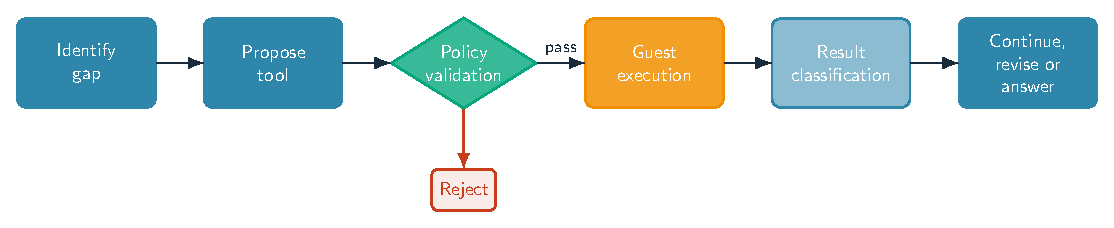
\includegraphics[width=0.95\linewidth]{Figures/fig_dynamic_tool_flow.pdf}
    \caption{Dynamic tool synthesis execution flow, showing the policy gate between tool proposal and guest execution.}
    \label{fig:dynamic_tool_flow}
\end{figure}

\fref{fig:dynamic_tool_flow} captures the six-stage execution loop described above.

\section{Ephemeral Sandboxing}
All executions of dynamic tools for each evaluation session can run in an
ephemeral sandboxed microVM. This creates a barrier to prevent cross-tool
contamination; to prevent persistent state abuse; to prevent memory poisoning.
The host will destroy the guest state after the execution of each evaluation and
store only pre-approved artifacts/logs/benchmark outputs.

A microVM backed task has the following life cycle:
\begin{enumerate}
    \item Allocate/resume guest image.
    \item Establish vsock transport.
    \item Send execution request/input bundle.
    \item Enforce timeout/output limit on host side.
    \item Receive/validate response from guest.
    \item Copy out validated approved artifacts.
    \item Destroy/reset guest state.
\end{enumerate}

For resume from snapshot, if used, reduces the start up time. However, it must be
used with caution. A valid snapshot must represent the original base state prior
to the generation of task specific secret files/tools and/or previous generated
tools. For evaluations that are at risk, use a completely new guest as it will
provide the most clear separation between tasks.

\begin{figure}[htbp]
    \centering
    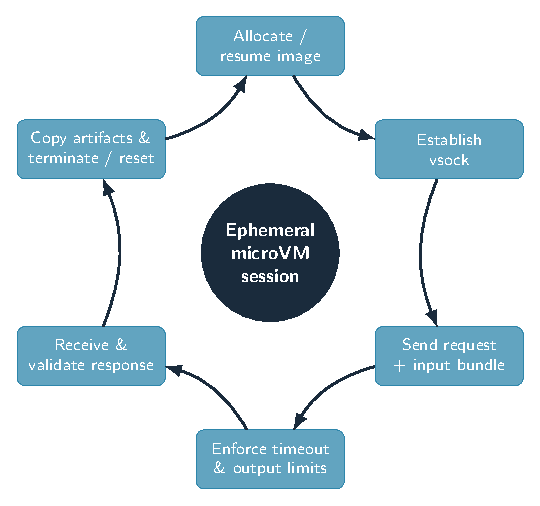
\includegraphics[width=0.8\linewidth]{Figures/fig_microvm_lifecycle.pdf}
    \caption{Lifecycle of an ephemeral microVM-backed tool execution session.}
    \label{fig:microvm_lifecycle}
\end{figure}

\fref{fig:microvm_lifecycle} shows the lifecycle of an ephemeral session.

The Host Daemon, Guest Runtime, Protocol Boundary, Dynamic Execution Engine,
MicroVM Lifecycle, Policy Model, and Failure-Handling Strategy are all defined in
this chapter. In the next chapter we will describe the evaluation method for the
system.

\section{Failure Modeling}
The failures that occur during the operation of the micro-vm are a key part of how ironclaw operates. Therefore when generating tools for the user they can fail to compile; time-out; generate incorrect results (provide invalid output); or attempt to execute malicious code. For every type of failure ironclaw will capture the specific failure classification with respect to the tool being executed, so the next process is done without exposing the host to the risk associated with that particular failure.

\section{Operational Considerations}
In addition to tracking which application was requested based on the unique id of the request; what policy decision was made at that time; what the duration of the execution was; what the final exit status was of the last task executed; and whether there were any truncations in the output. The guest should not log anything but information related to executing tasks. Also the guest should not have access to any secret information from the host. All this information is helpful for debugging; benchmarking; and security audits; none of them would violate the isolation boundaries.

% Chapter 4

\chapter{Methodology and Evaluation Protocol}
\label{Chapter4}
\lhead{Chapter 4. \emph{Methodology and Evaluation Protocol}}

\section{Experimental Design}
The evaluation is designed to allow for the independent measurement of three
claims; namely utility, security and systems performance. The utility aspects are
evaluated by comparing agents that must author task logic inline against agents
that can register and reuse that logic as a dynamic tool. The security aspects are tested through
attempting to breach containment generated by the use of an adversarially
created codebase. Finally, the performance characteristics of moving the
execution point of a process-level sandbox into a Firecracker microVM are
measured. Figure 4.1 describes the three independent evaluation axes used in the
evaluation.

\begin{figure}[htbp]
    \centering
    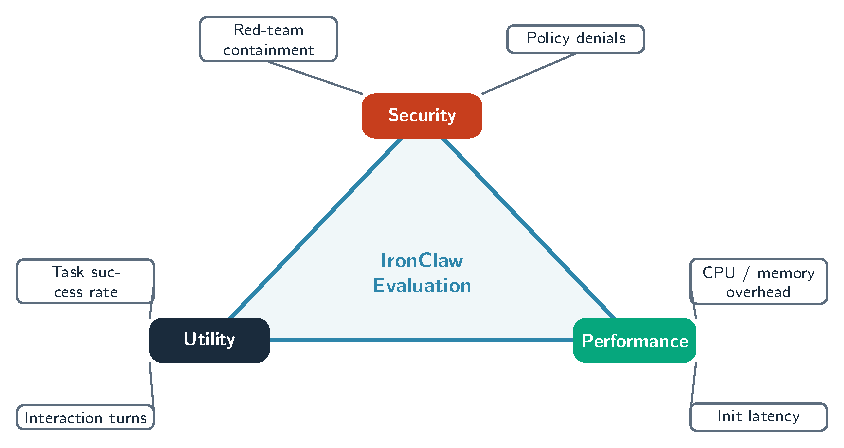
\includegraphics[width=0.85\linewidth]{Figures/fig_evaluation_pillars.pdf}
    \caption{Evaluation methodology overview: utility, security, and performance experiments are run independently and together answer the thesis research questions.}
    \label{fig:evaluation_pillars}
\end{figure}

\section{Baselines}
The two hypotheses require different matched baselines.

\noindent\textbf{H1 baseline:} an agent with generic SQL or sandboxed-script
capabilities that must author the required task logic inline for every request.
The H1 target receives the same capabilities plus runtime tool registration and
an explicit reuse policy.

\noindent\textbf{H2 baseline:} an ordinary child process executing the same
generated shell payload with the invoking user's view of host resources. The H2
target executes that payload inside IronClaw's Firecracker guest through the
authenticated vsock tool path.

\section{Utility and Security Evaluation}
Utility is evaluated using deterministic SQL, legacy-parser, and repository
compliance tasks. Metrics include answer correctness, model steps,
tool calls, billed input and output tokens, reasoning tokens, authored code, and
wall-clock time. Repetitive and mixed workloads isolate whether the one-time
creation cost is amortized.

Security is evaluated with five non-destructive host-resource attacks covering
file confidentiality, file integrity, environment confidentiality, device
visibility, and process-namespace visibility. A payload is contained only when
the targeted host resource remains unobserved and unmodified. The acceptance
criterion is zero successful accesses in the microVM condition.

\begin{figure}[htbp]
    \centering
    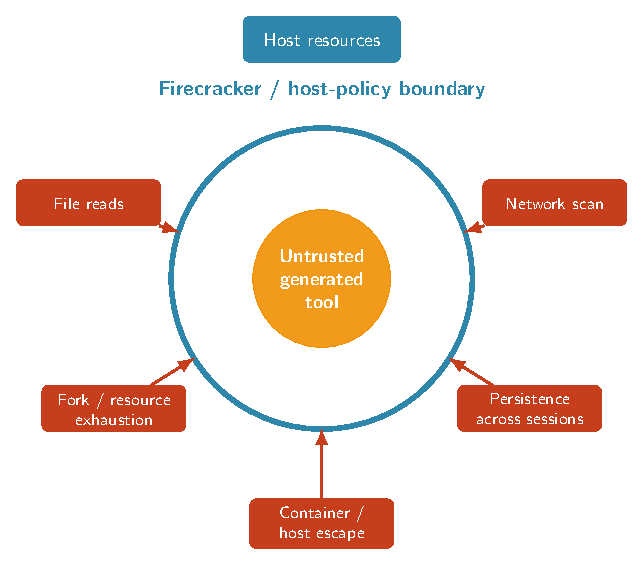
\includegraphics[width=0.9\linewidth]{Figures/fig_threat_model.pdf}
    \caption{Containment boundary for malicious synthesized tools. Attack vectors are blocked by the Firecracker and host-policy boundary.}
    \label{fig:threat_model}
\end{figure}

\fref{fig:threat_model} illustrates the containment boundary that the red-team
suite is designed to test.

\section{Performance Profiling}
Performance profiling measures:
\begin{itemize}
    \item process creation and microVM cold initialization latency;
    \item warm guest execution latency over an authenticated vsock session;
    \item host resident memory and configured guest memory;
    \item CPU time and utilization for a bounded workload; and
    \item stop, restart, authentication, and successful-probe recovery time.
\end{itemize}

The initialization target is $<500$\,ms for snapshot-resumed guests. Cold boot is
reported separately and does not test that target. Ten cold starts, twenty warm
executions, and five recovery trials are used in Chapter~\ref{ChapterH2}.

\begin{figure}[htbp]
    \centering
    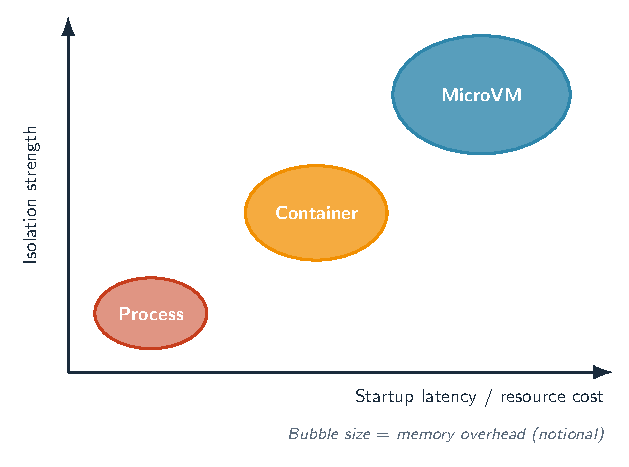
\includegraphics[width=0.85\linewidth]{Figures/fig_sandbox_comparison.pdf}
    \caption{Conceptual trade-off between isolation strength and runtime cost across the three execution modes compared in this thesis.}
    \label{fig:sandbox_comparison}
\end{figure}

Figure 4.3 shows how a tradeoff between Isolation Strength and Runtime Cost can
be expected.

% Chapter 5

\chapter{Implementation}
\label{Chapter5}
\lhead{Chapter 5. \emph{Implementation}}
\sloppy

\section{Repository and Source Availability}
The IronClaw implementation is maintained as a Rust workspace. The project is
hosted at:
\begin{center}
\url{https://github.com/suryavirkapur/ironclaw}
\end{center}

The local repository is organized around a host daemon, a guest runtime, shared
protocol and transport crates, tool implementations, security helpers, memory
support, channel integrations, configuration files, Firecracker build assets,
and smoke-test scripts. This structure keeps the host-facing control plane
separate from the guest execution plane.

\section{Workspace Organization}
The core workspace directories are:
\begin{itemize}
    \item \texttt{crates/ironclawd}: the host daemon, API server, agent loop,
    sandbox manager, provider integration, channel integration, and dispatch
    logic.
    \item \texttt{crates/irowclaw}: the guest runtime that executes inside the
    sandbox boundary and handles tool execution requests.
    \item \texttt{crates/common}: shared configuration structs, protobuf
    bindings, Firecracker abstractions, codec, transport traits, and stream
    transport.
    \item \texttt{crates/tools}: concrete tool implementations such as
    workspace-bounded file read/write, restricted shell execution, and browser
    automation.
    \item \texttt{crates/memory}: SQLite-backed memory, markdown indexing,
    hybrid retrieval, redaction, and pinned memory operations.
    \item \texttt{crates/security}: authentication, pairing, and rate-limiting
    components used by external control surfaces.
    \item \texttt{crates/channels}: messaging channel integrations.
    \item \texttt{configs/}: host and guest TOML configuration files.
    \item \texttt{scripts/}: root filesystem build scripts and smoke tests for
    local, container, websocket, and Firecracker paths.
\end{itemize}

\section{Host Configuration}
The host daemon is configured through \texttt{configs/ironclawd.toml}. The file
selects the execution mode, sandbox runtime, guest protocol, API bind address,
LLM provider endpoint, Firecracker assets, container runtime settings, daemon
log files, and channel integration settings. A representative excerpt is:
\begin{verbatim}
execution_mode = "auto"
sandbox_runtime = "container"
guest_protocol = "proto"
idle_timeout_minutes = 5
log_level = "info"

[server]
bind = "127.0.0.1"
port = 9938

[llm]
model = "glm-5.2"
base_url = "https://opencode.ai/zen/go/v1"
api = "chat_completions"

[firecracker]
enabled = false
kernel_path = "kernels/firecracker/vmlinux-6.1.155.bin"
rootfs_path = "rootfs/build/guest-rootfs.ext4"
api_socket_dir = "/tmp/ironclaw-fc"
vsock_uds_dir = "/tmp/ironclaw/vsock"
vsock_port = 5000

[container]
engine = "docker"
image = "ironclaw/irowclaw:latest"
network = "bridge"
brain_mount_path = "/mnt/brain"
command = ["irowclaw"]
\end{verbatim}

The configuration maps directly to strongly typed Rust structures in
\texttt{crates/common/src/config.rs}. The host supports multiple execution
modes: \texttt{auto}, \texttt{host\_only}, \texttt{guest\_tools}, and
\texttt{guest\_autonomous}. It also supports multiple sandbox runtime choices:
\texttt{auto}, \texttt{process}, \texttt{container}, and \texttt{microvm}. This
allows the same higher-level agent loop to be evaluated under different
containment strategies.

\section{Guest Configuration}
The guest runtime is configured with \texttt{irowclaw.toml}, normally mounted at
\texttt{/mnt/brain/config/irowclaw.toml}. The default guest configuration keeps
shell access disabled and allows file tools:
\begin{verbatim}
default_agent = "default"
log_level = "info"

[tools]
allow_bash = false
allow_file = true

[browser]
headless = true
timeout_ms = 30000
allowed_domains = []
max_memory_mb = 512
max_cpu_seconds = 20

[indexing]
max_chunk_bytes = 2048
embedding_model = "text-embedding-3-small"
vector_weight = 0.7
keyword_weight = 0.3
embedding_cache_size = 1000

[scheduler]
jobs_path = "/mnt/brain/cron/jobs.toml"
\end{verbatim}

For controlled testing, \texttt{configs/irowclaw.allow-bash.toml} enables the
shell tool and sets \texttt{allowed\_domains = ["*"]}. This is useful for
development and red-team experiments, but the safer default keeps network and
shell authority narrow.

\section{Protocol and Framing}
Host and guest communicate using a protobuf message envelope defined in
\texttt{crates/common/proto/ironclaw.proto}. Each message carries
\texttt{user\_id}, \texttt{session\_id}, \texttt{msg\_id},
\texttt{timestamp\_ms}, and a \texttt{cap\_token}. The payload is a protobuf
\texttt{oneof} that can represent authentication, agent control, user messages,
tool calls, tool responses, file operations, scheduler events, or streaming
deltas.

The current envelope supports:
\begin{itemize}
    \item \texttt{AuthChallenge} and \texttt{AuthAck} for guest authorization;
    \item \texttt{AgentControl} and \texttt{AgentState} for sleep/wake control;
    \item \texttt{UserMessage} for user-originated text;
    \item \texttt{ToolCallRequest} and \texttt{ToolCallResponse} for tool
    execution;
    \item \texttt{FileOpRequest} and \texttt{ToolResult} for bounded file
    operations;
    \item \texttt{JobTrigger} and \texttt{JobStatus} for scheduler integration.
\end{itemize}

The protobuf bytes are length-prefixed by \texttt{ProtoCodec}. The codec writes
a four-byte big-endian frame length followed by the encoded protobuf payload.
This same codec is used over in-memory local transport, child-process standard
I/O, and stream transports such as Firecracker vsock. Keeping framing separate
from the transport lets IronClaw test protocol behavior without requiring a
microVM for every unit test.

\begin{figure}[htbp]
    \centering
    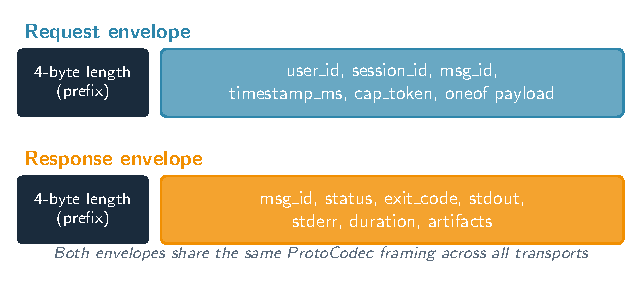
\includegraphics[width=0.95\linewidth]{Figures/fig_protocol_envelope.pdf}
    \caption{Host/guest protobuf message envelope used for all execution requests and responses.}
    \label{fig:protocol_envelope}
\end{figure}

\fref{fig:protocol_envelope} shows the request and response envelope structure.
\section{Authentication and Capability Handshake}
Prior to the runtime execution, the guest runtime will wait for an AuthChallenge
message from the host. The host then sends a capability token to the guest,
containing details regarding the authorization given to the runtime. Additionally,
the host also supplies the guest with a list of allowed tools and the preferred
mode of operation for the guest. After receiving this capability token, the guest
runtime will send an AuthAck message to confirm receipt of the token. Finally,
the guest will utilize the tool allow-list provided by the host to filter out
unauthorized tools from its ToolRegistry.

This capability-based handshaking method offers several important advantages to
this system: It gives the host one place to define session authority; It allows
for various methods to initiate the guest (different runtimes (e.g., process,
container, Firecracker)); It enables the guest to create all possible tools when
compiling its image prior to deployment and also gives the host complete control
of what tools are made accessible to the guest during each individual session.

\section{Sandbox Runtime Implementations}
\texttt{fire-cracker.rs} provides implementations for three sandbox abstractions:
\begin{itemize}
    \item VmManager: Manages VM Lifecycle (Start/Stop), returns information about
    current state of the vm instance.
    \item GuestRuntime: Contains everything required to manage a sandboxed
    runtime. Returned by VmManager.
    \item Transport: Used to communicate between host and guest.
\end{itemize}

\subsection{Process Runtime}
Two forms of local transport exist for testing and rapid development
environments. Local transports have extremely low overhead relative to launching
a new container or creating a new Firecracker microVM. Local transports however
cannot provide the same degree of isolation offered by containers and
microVM's. For example, if you wanted to test generated code that was supposed
to execute in an untrusted environment, you would likely choose to use a
container or a microVM instead of a local transport.

\subsection{Container Runtime}
IronClawD’s container manager (found in
\texttt{ironclawd/src/sandbox.rs}) uses docker to launch the guest runtime within
a container. Prior to starting the guest runtime, the container manager executes
the following actions:
\begin{itemize}
    \item Sanitizes the container name from user ID.
    \item Places a copy of the user's per-user brain directory into the container.
    \item Configures communication between the host and guest by setting
    environmental variables:
    \begin{itemize}
        \item \texttt{IRONCLAW BRAIN ROOT}: The path representing the brain root
        for the user in the guest. This root contains all files associated with
        memory.
        \item \texttt{IROCLAW\_CONFIG}: The path where the guest can locate its
        configuration file.
    \end{itemize}
\end{itemize}

All communication between the host and container occur via standard input/output
streams utilizing ChildPipeTransport. Any errors produced by the container are
sent directly from the container's standard error output to the host. Since both
the container and processes executing on the shared kernel space of the host
share their kernel space, it is generally accepted as being a less secure
boundary than that defined by microVM.

\subsection{Firecracker Runtime}
The Firecracker Manager (located in \texttt{ironclawd/src/sandbox.rs}) manages
Firecrackers creation and start-up process. Creation involves locating/building
kernels and root filesystems images, brain disk images, API socket and vsock
endpoint images. After creation, a Firecracker process spawns and waits for a
socket connection to an API socket. Once connected, Firecracker can be configured
with multiple API calls.

In addition to spawning a process, configuration for Firecracker's microVM can
be accomplished via specifying boot arguments. Some examples of boot arguments
include:
\begin{itemize}
    \item \texttt{console=ttyS0}: Directs console output to \texttt{/dev/ttyS0}.
    \item \texttt{panic=1}: If a fatal error occurs in the microVM, Firecracker
    immediately panics and exits.
    \item \texttt{pci=off}: Disallows enumeration of PCI devices in the microVM.
    \item \texttt{nomodules}: Disables module loading in the kernel.
    \item \texttt{root=/dev/vda}: Indicates that \texttt{/dev/vda} is mounted at
    root (/).
    \item \texttt{init=/init}: Tells init that it should call itself after
    mounting \texttt{/proc /sys /etc}...
\end{itemize}
Boot arguments are supplied to Firecracker via \texttt{--kernel-bootargs}.

Once InstanceStart has been successfully completed by the Firecracker manager, the host attempts to connect to a vsock unix domain socket (vsock:///unix/path/to/socket). The Firecracker manager had previously established a vsock device with guestCID 3. Once connected, the host issues a CONNECT command to establish a stream. In order for this connection attempt to succeed, the guest must listen on a vsock port (which is identified via a command line argument: \texttt{IRONCLAW\_VSOCK=1}) once it reaches InstanceStart.

Once a successful OK response is received from the guest runtime after sending a CONNECT command, the host wraps the stream in StreamTransport and continues to send/receive commands/envelopes as it would with other runtimes.

\section{Guest Runtime Inner Loop}
The guest runtime performs an initialization process which includes:
\begin{itemize}
    \item reading configuration data from \texttt{config.json}
    \item setting up logging
    \item creating directories for brains
    \item opening a sqlite database
    \item initializing memory schema
    \item create a workspace directory
    \item register the tools
    \item enter the transport loop
\end{itemize}

The default path for brain directories is \texttt{/mnt/brain}. The default path
for the workspace is \texttt{/mnt/brain/workspace}. All file-based tools live in
the Workspace Directory.

The runtime loop uses \texttt{tokio::select!} to allow concurrent handling of
both Host messages and Scheduler events. Additionally, a simple power state is
stored to \texttt{config/agent\_state.toml}. Messages sent by agentcontrol can put
the guest runtime into a sleeping state or wake the guest Runtime out of its
sleeping state. While the runtime is sleeping, user messages that request tool
Invocation will receive an explicit rejection message.

First, local memory commands contained within user messages are processed.
Second, prompts are injected and policies are checked. Based upon the execution
mode chosen (the type of Execution allowed), it will send a notification to the
Host that execution in the guest is prohibited, Request that the Host choose a
tool invocation for planning purposes, or execute autonomously with a simple
planner.

\section{Tool Registry and Tool Implementations}
Tools that exist in the guest register themselves in a \texttt{ToolRegistry}.
Although registration and authorization are now separate; although a tool may be
registered in the registry, it will still be denied Unless the name of the tool
exists in the Host's provided Allow-List.

File-based tools utilize a Rooted Path Resolver. Any absolute path (which includes
Parent-Directories) and Platform Specific Prefixes are not permitted as they
would potentially be used to attempt escapes from the Workspace Root such as
\texttt{../../etc/passwd}.

The Restricted Shell Tool executes commands via \texttt{sh -lc} inside the
Workspace Directory. Obvious High-Risk Substrings (such as \texttt{sudo},
\texttt{curl}, \texttt{wget}, \texttt{ssh}, \texttt{scp}, \texttt{nc},
\texttt{netcat}, \texttt{file://}, \texttt{data:}, and \texttt{javascript:}) are
blocked. Output is capped at 32 KiB and Truncated if necessary. Note: these
Safety Checks do not replace Micro VM Isolation; they are defense in Depth
within the guest.

The Browser Tool Launches a Headless Chromium-Compatible Web-Browser. It supports
Fetch requests and screenshot requests as well as JavaScript Evaluation
Requests. It validates url schemes, blocks URLs starting with \texttt{file:},
\texttt{data:}, and \texttt{javascript:}, requires http(s) scheme, enforces a
list of allowable domains, applies some process Limits and expects a timeout.
Screenshot Results returned are encoded as base64 Strings.

\section{Memory and Scheduler Integration}
The guest runtime creates a sqlite backed memory store and then Uses Hybrid
Retrieval over markdown Chunks. Configuration controls chunk size, Embedding
Model, vector weight, Keyword Weight, and Embedding Cache Size. The memory
commands provide explicit pinned memory insertion, listing and Forgetting.
Secrets are redacted before user-provided memories are stored.

The scheduler reads jobs from \texttt{/mnt/brain/cron/jobs.toml}. Scheduler
triggers are converted into protocol messages so that the same transport path
can be utilized for scheduled work and Interactive Work. A scheduled job can
awaken a sleeping runtime and instead of dumping unbounded Output into the
message stream return a log reference.

\section{Security Checks and Output Sanitization}
A layer of safety has been implemented by the guest prior to executing each tool.
The inputs have been checked for patterns of prompt-injectable attacks and Policy
violations. The outputs have been checked for possible leaks before being
returned. This provides ironclaw multiple gates: Host-side Policy before
dispatch, guest-side Policy before execution, tool-specific restrictions during
execution and outbound sanitization after execution.

\section{Testing and Smoke Scripts}
Testing exists in the Codebase for all of the following: Runtime Configuration;
Vsock Transport; Scheduler Behavior; safety handling; browser behavior; Sandbox
Runtime Behavior; Webhook Handling; Channel Handling; Daemon Lifecycle; core
protocol modules.

Smoke Scripts located under \texttt{scripts/} test major deployment paths:
\begin{enumerate}
    \item \texttt{Smoke-local-guest.sh}: test local guest path;
    \item \texttt{Smoke-firecracker.sh}: test firecracker boot path;
    \item \texttt{Smoke-firecracker-ws.sh}: test Firecracker Websocket Path;
    \item \texttt{smoke-guest-tools-ws.sh}: test guest tool path using websocket;
    \item \texttt{build-guest-rootfs.sh}: build guest root file system.
\end{enumerate}

\fussy

% Chapter 6

\chapter{Conclusion and Future Work}
\label{Chapter6}
\lhead{Chapter 6. \emph{Conclusion and Future Work}}

\section{Contributions}
This research provides a practical architecture that integrates dynamic tool synthesis into micro-VM isolations. This is the first significant contribution -- just enabling an agent to generate code does not automatically place that code under a boundary that can be measured, destroyed, and replicated. Rather than simply evaluating the performance benefits of the system (i.e., utility), we will also measure the cost associated with isolating those tools from one another (i.e., isolation).

\section{Limitations}
Our evaluation has been constrained by our selection of benchmarks; the availability of machines to run these evaluations; and the quality of the large language model that was employed in each experiment. While dynamic tool synthesis likely will have the greatest impact on workflows that are heavy in data transformation, and thus require frequent use of tools created during the workflow, there are certainly many cases in which the fixed set of tools provided in an environment is sufficient. In addition to demonstrating containment of an untrusted tool against a predefined payload set, security testing can demonstrate that there are no vulnerabilities in the virtual machine monitor, kernel, or host integration.

\section{Future Directions}
There are four possible areas for extending IronClaw. First, the current suite of benchmarks could be extended to include larger, more realistic codebases, and/or longer running data processing jobs. Second, it should be possible to cache tools produced through dynamic tool synthesis with their corresponding signature and policies so that when an agent needs to perform a task again, they don't have to recreate all of the necessary tools. Third, we could expand our security evaluation to include fuzzing and kernel level instrumentation. Finally, we could extend the system to allow users to specify richer policies for defining network, file, CPU, memory, time limits for each dynamically generated tool.

\section{Conclusion}
Ultimately, dynamic tool synthesis is a natural extension of the ability for autonomous agents to create new capabilities at runtime. However, without a well-defined runtime boundary around such synthesized code creation, this increased flexibility comes at too great a risk. Thus, IronClaw demonstrates how Firecracker's microVMs can be used as a viable solution for creating a reasonable level of isolation for untrusted agent-created tools while still providing a way to evaluate the utility and performance impacts of using such tools.

\section{Summary}
In this Chapter, I briefly summarized my expected contributions, limitations, future work, and conclusions based on this dissertation. The Appendices contain information about installing, compiling, executing and configuring your environment in order to reproduce my work.

%\input{Chapters/Chapter7}

%-------------------------------------------------------------------------------
%	THESIS CONTENT - APPENDICES
%-------------------------------------------------------------------------------

\addtocontents{toc}{\vspace{2em}} % Add a gap in the Contents, for aesthetics

\appendix % Cue to tell LaTeX that the following 'chapters' are Appendices

% Include the appendices of the thesis as separate files from the Appendices
% folder
% Uncomment the lines as you write the Appendices

% Appendix A

\chapter{Installation and Execution Instructions}
\label{AppendixA}
\lhead{Appendix A. \emph{Installation and Execution Instructions}}

\section{Submitted Folders and Files}
The submitted project package should include the following folders and files:
\begin{itemize}
    \item \texttt{crates/}: Rust workspace crates for the host daemon, guest
    runtime, shared protocol, security, memory, tools, heartbeat, and channels.
    \item \texttt{configs/}: runtime configuration files for IronClaw and the
    guest runtime.
    \item \texttt{scripts/}: build and smoke-test scripts for local and
    Firecracker-backed execution.
    \item \texttt{rootfs/}: guest root filesystem skeleton files.
    \item \texttt{kernels/firecracker/}: kernel images used by the Firecracker
    runtime.
    \item \texttt{docs/}: supporting architecture and setup documentation.
    \item \texttt{experiments/}: H1 TypeScript harness, deterministic fixtures,
    raw JSON results, and rendered H1/H2 result reports.
    \item \texttt{Report Thesis Suryavir Kapur/}: thesis report source and
    generated PDF.
\end{itemize}

\section{Prerequisites}
The development machine should have Rust installed through \texttt{rustup}, the
toolchain specified in \texttt{rust-toolchain.toml}, \texttt{cargo},
\texttt{make}, a Linux environment capable of running Firecracker, and LaTeX
tools for building the report. Firecracker execution may require KVM support and
appropriate permissions on the host.

\section{Compilation Steps}
From the repository root, build the Rust workspace using:
\begin{verbatim}
cargo build --workspace
\end{verbatim}

Run the test suite using:
\begin{verbatim}
cargo test --workspace
\end{verbatim}

Check every feature and target, including the Firecracker evaluation example:
\begin{verbatim}
cargo check --workspace --all-targets --all-features
\end{verbatim}

Build the thesis PDF from the report directory using:
\begin{verbatim}
cd "Report Thesis Suryavir Kapur"
make
\end{verbatim}

\section{Execution Steps}
Local smoke tests can be executed using the scripts under \texttt{scripts/}.
Typical commands include:
\begin{verbatim}
./scripts/smoke-local-guest.sh
./scripts/smoke-firecracker.sh
./scripts/smoke-firecracker-ws.sh
./scripts/smoke-guest-tools-ws.sh
\end{verbatim}

Configuration files under \texttt{configs/} select the runtime behavior,
permissions, and guest execution mode. Before running Firecracker tests, verify
that the configured kernel path, root filesystem path, vsock settings, and file
permissions match the local machine.

\section{Evaluation Reproduction}
Reproduce H1 from the \texttt{experiments/} directory:
\begin{verbatim}
export DEEPSEEK_API_KEY=...
npm install
npm run experiment
\end{verbatim}
This regenerates \texttt{RESULTS.md} and \texttt{results.json}. Individual
conditions can be selected, for example \texttt{npm run experiment -{}- E5:B}.

Reproduce H2 from the repository root on a Linux host with KVM, Firecracker,
the documented guest kernel, and the immutable Ubuntu root filesystem:
\begin{verbatim}
cargo run -p common --features firecracker \
  --example h2_security_performance
\end{verbatim}
This writes \texttt{experiments/H2\_RESULTS.md} and
\texttt{experiments/h2-results.json}.

\section{Configuration Details}
The main configuration files are:
\begin{itemize}
    \item \texttt{configs/ironclawd.firecracker.toml}: Firecracker-backed host
    daemon configuration.
    \item \texttt{configs/ironclawd.guest-tools.toml}: guest-tools execution
    mode.
    \item \texttt{configs/ironclawd.guest-autonomous.toml}: autonomous guest
    execution mode.
    \item \texttt{configs/irowclaw.allow-bash.toml}: guest runtime configuration
    that permits shell execution for controlled test scenarios.
\end{itemize}

\section{Reproducibility Checklist}
The final project package should make it possible to reproduce the implementation
and evaluation environment. Before submission, verify that:
\begin{itemize}
    \item the Rust workspace builds with \texttt{cargo build --workspace};
    \item the available automated tests run with \texttt{cargo test --workspace};
    \item configuration files under \texttt{configs/} match the local execution
    mode;
    \item Firecracker kernel and root filesystem paths are documented;
    \item smoke-test commands and expected outputs are recorded;
    \item H1 and H2 result JSON files can be regenerated with the commands above;
    \item generated report and presentation PDFs are included.
\end{itemize}

% Appendix B

\chapter{Draft Paper Outline}
\label{AppendixB}
\lhead{Appendix B. \emph{Draft Paper Outline}}

\section{Draft Title}
\textbf{IronClaw: Dynamic Tool Synthesis with Secure MicroVM Isolation for
Autonomous Agents}

\section{Draft Abstract}
Autonomous agents based on Large Language Models increasingly rely on external
tools to complete long-horizon software engineering, data processing, and
operational tasks. Fixed tool registries simplify control and auditing, but they
limit the agent when a task requires an unanticipated parser, transformation,
test harness, or integration. Dynamic tool synthesis addresses this limitation
by allowing the agent to generate executable code during a task, but doing so
introduces a severe security problem: generated code is untrusted and may be
incorrect, malicious, prompt-injected, or resource-exhaustive.

This paper will present IronClaw, a self-hosted agent platform that separates
trusted host control from untrusted guest execution. The host daemon manages
model interaction, policy, memory, configuration, and sandbox lifecycle, while a
guest runtime executes generated tools inside a restricted environment. The
system supports process, container, and Firecracker-backed microVM runtimes over
a shared protobuf protocol. The planned evaluation will compare fixed-tool and
dynamic-tool agents on multi-step tasks, measure containment against malicious
payloads, and quantify latency and resource overhead across sandbox backends.
The expected contribution is a practical architecture and empirical methodology
for making runtime tool synthesis useful without collapsing the host trust
boundary.

\section{Planned Paper Sections}
\begin{enumerate}
    \item \textbf{Introduction}
    \begin{itemize}
        \item Motivation for dynamic tool synthesis.
        \item Security risk of executing agent-generated code.
        \item Summary of IronClaw's host/guest architecture.
        \item Contributions and evaluation goals.
    \end{itemize}

    \item \textbf{Background and Related Work}
    \begin{itemize}
        \item LLM agents and tool use.
        \item Dynamic skill and tool acquisition.
        \item Sandboxing, containers, virtual machines, and microVMs.
        \item Firecracker and lightweight virtualization.
    \end{itemize}

    \item \textbf{Threat Model}
    \begin{itemize}
        \item Untrusted generated code.
        \item Prompt injection and malicious task data.
        \item Host filesystem, network, memory, and credential protection.
        \item Non-goals such as proving the absence of all hypervisor bugs.
    \end{itemize}

    \item \textbf{System Design}
    \begin{itemize}
        \item Host daemon responsibilities.
        \item Guest runtime responsibilities.
        \item Protobuf message envelope and capability handshake.
        \item Tool allowlists and policy gates.
        \item Runtime options: process, container, and microVM.
    \end{itemize}

    \item \textbf{Implementation}
    \begin{itemize}
        \item Rust workspace organization.
        \item Configuration model.
        \item Transport and framing.
        \item Firecracker manager and vsock setup.
        \item Tool registry, file tools, restricted shell, browser tool, memory,
        and scheduler.
    \end{itemize}

    \item \textbf{Evaluation Methodology}
    \begin{itemize}
        \item Utility benchmarks for fixed-tool versus dynamic-tool agents.
        \item Security red-team payload suite.
        \item Performance measurements for latency, CPU, memory, and startup.
        \item Reproducibility and environment details.
    \end{itemize}

    \item \textbf{Results}
    \begin{itemize}
        \item Task completion rate.
        \item Turn count and token usage.
        \item Containment outcomes.
        \item Runtime overhead comparisons.
    \end{itemize}

    \item \textbf{Discussion}
    \begin{itemize}
        \item When dynamic synthesis helps.
        \item When fixed tools are sufficient.
        \item Security and usability trade-offs.
        \item Operational limits of microVM-based isolation.
    \end{itemize}

    \item \textbf{Limitations}
    \begin{itemize}
        \item Benchmark representativeness.
        \item Hardware dependency.
        \item Model dependency.
        \item Scope of red-team payloads.
    \end{itemize}

    \item \textbf{Conclusion}
    \begin{itemize}
        \item Summary of architecture, measurements, and lessons.
        \item Future work on stronger policies, snapshots, caching, and broader
        benchmarks.
    \end{itemize}
\end{enumerate}

%\input{Appendices/AppendixC}

\addtocontents{toc}{\vspace{2em}} % Add a gap in the Contents, for aesthetics

\backmatter

%-------------------------------------------------------------------------------
%	BIBLIOGRAPHY
%-------------------------------------------------------------------------------

\label{Bibliography}

\lhead{\emph{Bibliography}} % Change the page header to say "Bibliography"

\bibliographystyle{plain}
\bibliography{Bibliography}

\end{document}
